En esta sección se presentan los resultados experimentales obtenidos para evaluar el rendimiento de los algoritmos presentados. Los resultados se resumen en las tablas a continuacion, armadas con los tiempos promedio en milisegundos [\textit{ms}] para cada categoría y diferentes tamaños de entrada. Para cada tamaño, se realizaron tres pruebas independientes (\textit{test1}, \textit{test2}, y \textit{test3}) cuyos valores se promediaron para destacar el comportamiento general del algoritmo. Los tiempos destacados en \textbf{negrita} representan los valores promedio obtenidos.

\subsubsection*{Fuerza Bruta}
La tabla muestra los resultados obtenidos al probar el algoritmo de fuerza bruta con diferentes tipos de casos. Este método, aunque simple en su concepto, examina todas las posibles formas de transformar una cadena en otra y elige la que tiene el menor costo. Sin embargo, debido a que utiliza recursión y tiene una complejidad exponencial, el tiempo que tarda en ejecutarse puede variar mucho dependiendo de la longitud y las características de las cadenas analizadas.

\begin{table}[h]
\centering
\scalebox{0.9}{
\begin{tabular}{c|ccccc}
& \textbf{Distinto Tam. [ms]} & \textbf{Str Iguales [ms]} & \textbf{1 Str Vacío [ms]} & \textbf{Distintos Str [ms]} & \textbf{Solo Transposición [ms]} \\ \hline
\textbf{5} & \textbf{0.209766667} & \textbf{0.2022} & \textbf{0.001} & \textbf{0.2143} & \textbf{0.206066667} \\ \hline
test1 & 0.1994 & 0.1985 & 0.001 & 0.2086 & 0.1988 \\
test2 & 0.2307 & 0.2036 & 0.0011 & 0.2351 & 0.1992 \\
test3 & 0.1992 & 0.2045 & 0.001 & 0.1992 & 0.1995 \\ \hline
\textbf{6} & \textbf{0.214666667} & \textbf{1.151733333} & \textbf{0.00166667} & \textbf{1.084166667} & \textbf{1.0974} \\ \hline
test1 & 0.2421 & 1.1352 & 0.001 & 1.0851 & 1.0847 \\
test2 & 0.1992 & 1.1225 & 0.0009 & 1.0812 & 1.1227 \\
test3 & 0.2081 & 1.1251 & 0.001 & 1.0814 & 1.1258 \\ \hline
\textbf{7} & \textbf{4.302233333} & \textbf{6.211533333} & \textbf{0.000966667} & \textbf{6.0378} & \textbf{6.062966667} \\ \hline
test1 & 6.9041 & 6.5234 & 0.001 & 6.448 & 6.4338 \\
test2 & 6.1986 & 6.077 & 0.001 & 6.4517 & 6.0974 \\
test3 & 5.9828 & 6.0432 & 0.001 & 6.4493 & 6.0722 \\ \hline
\textbf{8} & \textbf{14.01323333} & \textbf{34.0214} & \textbf{0.00133333} & \textbf{33.5678} & \textbf{35.26496667} \\ \hline
test1 & 5.0211 & 34.3423 & 0.0011 & 32.8275 & 33.8369 \\
test2 & 1.6996 & 33.1743 & 0.001 & 32.9435 & 34.9697 \\
test3 & 35.319 & 34.5429 & 0.0011 & 33.9435 & 34.9375 \\ \hline
\textbf{9} & \textbf{51.67986667} & \textbf{198.698} & \textbf{0.00113333} & \textbf{184.9345667} & \textbf{192.8536667} \\ \hline
test1 & 77.7683 & 222.328 & 0.001 & 185.553 & 190.984 \\
test2 & 74.2817 & 189.866 & 0.0011 & 185.829 & 182.521 \\
test3 & 2.9984 & 183.9 & 0.001 & 183.422 & 205.002 \\

\end{tabular}
}
\end{table}

\begin{figure}[H]
    \centering
    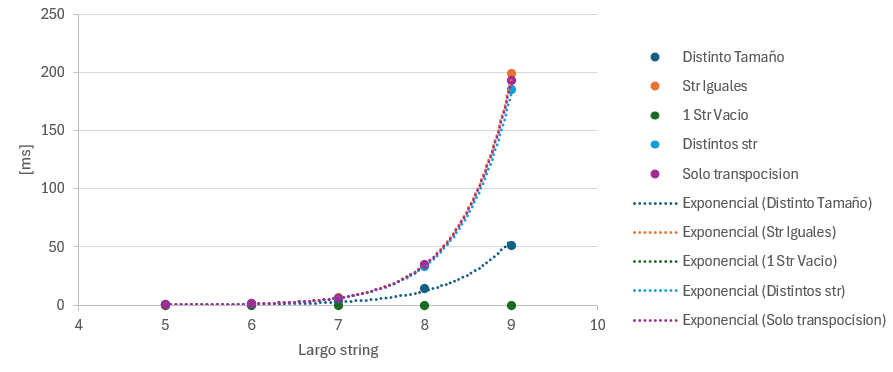
\includegraphics[width=1\linewidth]{AlgoReportTemplate-main//images/GraphBruteForce.png}
    \label{fig:enter-label}
\end{figure}
\vspace{5px}

\subsubsection*{Casos de prueba base}
Se utilizaron varios casos de prueba básicos para evaluar el rendimiento del código de programación dinámica. Estos casos consisten en diferentes configuraciones de entrada, donde se varían características clave del algoritmo. Los resultados de las pruebas se presentan en la siguiente tabla.
\begin{table}[h]
\centering
\scalebox{0.9}{
\begin{tabular}{c|l|c}

\textbf{Prueba} & \textbf{Cadenas} & \textbf{Resultado} \\ \hline
\textbf{1} & 
\begin{tabular}[c]{@{}l@{}}
\texttt{ } \\ 
\texttt{ } \\ 
\end{tabular} & \textbf{0} \\ \hline

\textbf{2} & 
\begin{tabular}[c]{@{}l@{}}
\texttt{nada} \\ 
\texttt{anda} \\ 
\end{tabular} & \textbf{1} \\ \hline

\textbf{3} & 
\begin{tabular}[c]{@{}l@{}}
\texttt{componentes} \\ 
\texttt{comerciales} \\ 
\end{tabular} & \textbf{10} \\ \hline

\textbf{4} & 
\begin{tabular}[c]{@{}l@{}}
\texttt{datos} \\ 
\texttt{estructuras} \\ 
\end{tabular} & \textbf{12} \\ \hline

\textbf{5} & 
\begin{tabular}[c]{@{}l@{}}
\texttt{hola} \\ 
\texttt{ } \\ 
\end{tabular} & \textbf{4} \\

\end{tabular}
}
\end{table}

\subsubsection*{Programacion Dinamica}

La tabla presenta los resultados experimentales obtenidos al aplicar el algoritmo basado en Programación Dinámica a distintos casos de prueba. Este enfoque optimiza el proceso de transformación al almacenar y reutilizar soluciones a subproblemas, lo que reduce significativamente la cantidad de cálculos redundantes en comparación con métodos más simples como el de fuerza bruta. Gracias a esta técnica, el algoritmo logra una complejidad polinómica, haciendo que su tiempo de ejecución sea mucho más eficiente, incluso para cadenas de mayor longitud o complejidad.

\begin{table}[h]
\centering
\scalebox{0.9}{
\begin{tabular}{c|ccccc}

& \textbf{Distinto Tam.} & \textbf{Str Iguales} & \textbf{1 Str Vacío} & \textbf{Distintos Str} & \textbf{Solo Transposición} \\ \hline
\textbf{5} & \textbf{0.0132} & \textbf{0.013033333} & \textbf{0.009566667} & \textbf{0.011733333} & \textbf{0.0104} \\ \hline
test1 & 0.0145 & 0.0132 & 0.0108 & 0.0144 & 0.0111 \\
test2 & 0.0101 & 0.0113 & 0.005 & 0.0104 & 0.0111 \\
test3 & 0.0131 & 0.0121 & 0.0114 & 0.0105 & 0.011 \\ \hline
\textbf{6} & \textbf{0.011733333} & \textbf{0.012066667} & \textbf{0.008933333} & \textbf{0.0131} & \textbf{0.012466667} \\ \hline
test1 & 0.0121 & 0.0122 & 0.0101 & 0.0141 & 0.0114 \\
test2 & 0.0102 & 0.0115 & 0.008 & 0.011 & 0.0115 \\
test3 & 0.0131 & 0.0124 & 0.0099 & 0.0119 & 0.013 \\ \hline
\textbf{7} & \textbf{0.024733333} & \textbf{0.012066667} & \textbf{0.009133333} & \textbf{0.013133333} & \textbf{0.013766667} \\ \hline
test1 & 0.0319 & 0.0131 & 0.011 & 0.0152 & 0.0143 \\
test2 & 0.0112 & 0.0122 & 0.008 & 0.012 & 0.0115 \\
test3 & 0.0106 & 0.0116 & 0.009 & 0.015 & 0.0132 \\ \hline
\textbf{8} & \textbf{0.014833333} & \textbf{0.014333333} & \textbf{0.010333333} & \textbf{0.013066667} & \textbf{0.015033333} \\ \hline
test1 & 0.0112 & 0.0146 & 0.0101 & 0.0128 & 0.0143 \\
test2 & 0.0123 & 0.014 & 0.0099 & 0.0125 & 0.0139 \\
test3 & 0.0131 & 0.0143 & 0.0098 & 0.013 & 0.0147 \\ \hline
\textbf{9} & \textbf{0.0132} & \textbf{0.0146} & \textbf{0.0114} & \textbf{0.015} & \textbf{0.020866667} \\ \hline
test1 & 0.013 & 0.0143 & 0.0108 & 0.0149 & 0.0238 \\
test2 & 0.0129 & 0.0139 & 0.011 & 0.0126 & 0.0166 \\
test3 & 0.0111 & 0.0168 & 0.0107 & 0.0162 & 0.0222 \\

\end{tabular}
}
\end{table}

\begin{figure}[H]
    \centering
    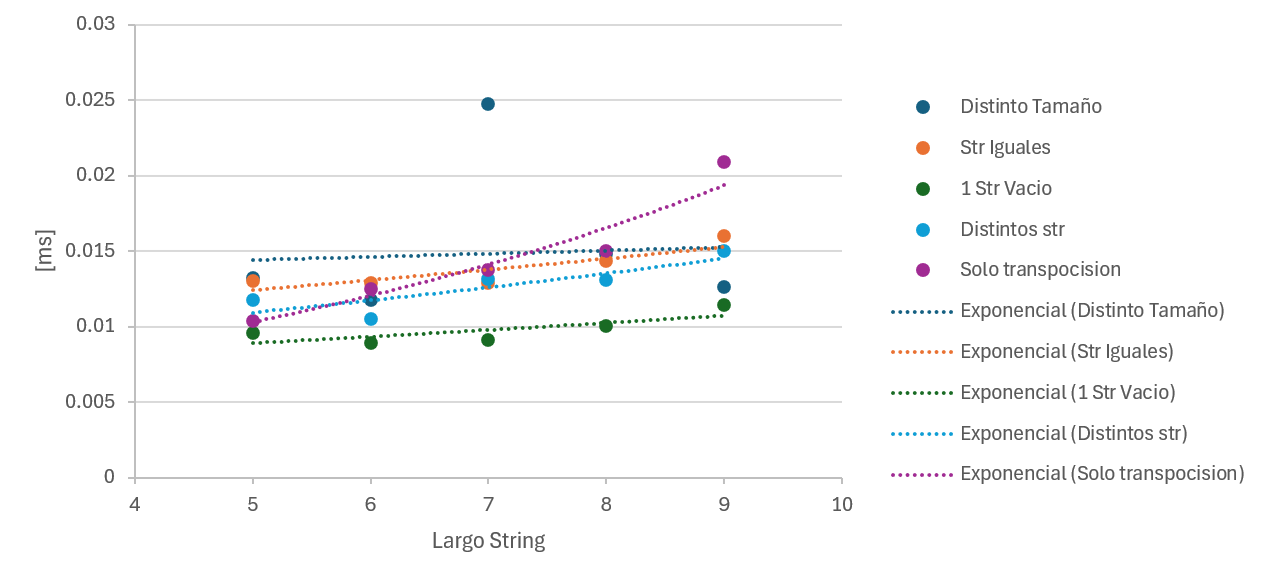
\includegraphics[width=1\linewidth]{AlgoReportTemplate-main//images/graphDP.png}
    \label{fig:enter-label}
\end{figure}

\subsubsection*{Casos de prueba base}

Al igual que en el caso de la fuerza bruta, se evaluo el codigo frente a casos de prueba bases, en los que se variaban caracteristicas importantes del codigo.
Los resultaos se prensentan en la siguiente tabla.

\begin{table}[h]
\centering
\scalebox{0.9}{
\begin{tabular}{c|l|c}

\textbf{Prueba} & \textbf{Cadenas} & \textbf{Resultado} \\ \hline
\textbf{1} & 
\begin{tabular}[c]{@{}l@{}}
\texttt{ } \\ 
\texttt{ } \\ 
\end{tabular} & \textbf{0} \\ \hline

\textbf{2} & 
\begin{tabular}[c]{@{}l@{}}
\texttt{nada} \\ 
\texttt{anda} \\ 
\end{tabular} & \textbf{1} \\ \hline

\textbf{3} & 
\begin{tabular}[c]{@{}l@{}}
\texttt{componentes} \\ 
\texttt{comerciales} \\ 
\end{tabular} & \textbf{10} \\ \hline

\textbf{4} & 
\begin{tabular}[c]{@{}l@{}}
\texttt{datos} \\ 
\texttt{estructuras} \\ 
\end{tabular} & \textbf{12} \\ \hline

\textbf{5} & 
\begin{tabular}[c]{@{}l@{}}
\texttt{hola} \\ 
\texttt{ } \\ 
\end{tabular} & \textbf{4} \\

\end{tabular}
}
\end{table}